\chapter{Circuit Analysis}
\label{chapter:circuits}



\section{Electric Current}

In an electric circuit, a large number of charge ``carriers'' are pushed along
by a small electrostatic force in a conductive material, creating an
\textbf{electric current}. We can model positive charges moving from the
positive terminal towards the negative terminal, as shown in
Fig.~\ref{fig:current}.
\begin{figure}[ht]
  \centering
  \begin{tikzpicture}[scale=.8,thick]
    \fill[gray!30] rectangle (7,3);
    \draw[very thick] (0,0)--(7,0);
    \draw[very thick] (0,3)--(7,3);

    \begin{scope}[magenta]
      \draw[fill=magenta!10] (1,.5) circle (.25) node{$+$};
      \draw[axes] (1.25,.5)--(1.75,.5);

      \draw[fill=magenta!10] (3,.75) circle (.25) node{$+$};
      \draw[axes] (3.25,.75)--(3.75,.75);

      \draw[fill=magenta!10] (6,1.75) circle (.25) node{$+$};
      \draw[axes] (6.25,1.75)--(6.75,1.75);

      \draw[fill=magenta!10] (5,2.5) circle (.25) node{$+$};
      \draw[axes] (5.25,2.5)--(5.75,2.5);

      \draw[fill=magenta!10] (4,1.75) circle (.25) node{$+$};
      \draw[axes] (4.25,1.75)--(4.75,1.75);

      \draw[fill=magenta!10] (5.25,1) circle (.25) node{$+$};
      \draw[axes] (5.5,1)--(6,1);

      \draw[fill=magenta!10] (2,1.5) circle (.25) node{$+$};
      \draw[axes] (2.25,1.5)--(2.75,1.5);

      \draw[fill=magenta!10] (.5,2.5) circle (.25) node{$+$};
      \draw[axes] (.75,2.5)--(1.25,2.5);

      \draw[fill=magenta!10] (2.5,2.25) circle (.25) node{$+$};
      \draw[axes] (2.75,2.25)--(3.25,2.25);
    \end{scope}

    \node at (0,1.5)[left] {\huge$+$};
    \node at (7,1.5)[right]{\huge$-$};
  \end{tikzpicture}
  \caption{Model of positive charges moving from the positive towards
    the negative terminal}
  \label{fig:current}
\end{figure}

The \textbf{electric current} is defined as the rate at which \textbf{charges}
$Q$ pass through a point in a circuit. In differential form, it is expressed as
a function of time:
\begin{important-equation}
  I(t)=\diff Qt %= \frac QV\diff Vt = (ne)(Av_d)
  \label{eq:current}
\end{important-equation}
The SI unit for electric current is an \emph{amp\`{e}re} (\si\ampere), and is
one of the seven base SI unit. (The origin of the definition of an amp\`{e}re
of current was discussed in Chapter~\ref{chapter:magnetism1}.) The SI unit for
electrical charge, a \emph{coulomb}, is therefore defined as the amount of
charge that \SI1{\ampere} of current passes through a circuit in \SI1\second,
i.e.:
\begin{equation*}
  \SI1\coulomb=\SI1{\ampere\second}
\end{equation*}


\subsection{Direct Current}
In a \textbf{direct current} (\textbf{DC}), the flow of charges is always in
the same direction, but the current itself does not have to be constant in
time. The examples in Fig.~\ref{fig:DC-examples} shows different types of
direct currents. Circuits with only resistors has constant, time-independent
current, like in Fig.~\ref{fig:resistive-dc}. Circuits with charging or
discharging capacitors have an exponentially decaying current, as shown in
Fig.~\ref{fig:capacitive-dc}. Circuit with capacitors and inductors has a
current that has a sinusoidal component, as shown in
Fig.~\ref{fig:unductive-dc}.
\begin{figure}[ht]
  \centering
  \begin{subfigure}{.28\textwidth}
    \centering
    \begin{tikzpicture}[scale=.8]
      \draw[red,ultra thick] (0,3)--(4,3);
      \draw[axes] (0,0)--(4,0) node[right]{$t$};
      \draw[axes] (0,0)--(0,4) node[above]{$I$};
    \end{tikzpicture}
    \caption{Resistive circuits}
    \label{fig:resistive-dc}
  \end{subfigure}
  \begin{subfigure}{.34\textwidth}
    \centering
    \begin{tikzpicture}[scale=.8]
      \draw[smooth,samples=20,domain=0:3.5,function]
      plot(\x,{3*(exp(-.8*\x))});
      \draw[axes] (0,0)--(4,0) node[right]{$t$};
      \draw[axes] (0,0)--(0,4) node[above]{$I$};
    \end{tikzpicture}
    \caption{Resistive \& capacitive circuits}
    \label{fig:capacitive-dc}
  \end{subfigure}
  \begin{subfigure}{.34\textwidth}
    \centering
    \begin{tikzpicture}[scale=.8]
      \draw[axes] (0,0)--(4,0) node[right]{$t$};
      \draw[axes] (0,0)--(0,4) node[above]{$I$};
      \draw[smooth,samples=20,domain=0:3.5,function]
      plot(\x,{sin(120*\x)+2});
    \end{tikzpicture}
    \caption{Capacitive \& inductive circuits}
    \label{fig:unductive-dc}
  \end{subfigure}
  \caption{Examples of direct-current circuits}
  \label{fig:DC-examples}
\end{figure}



\subsection{Alternating Current}

In contrast, in an \textbf{alternating current} (\textbf{AC}), the flow of
charges changes direction, usually as a sinusoidal function of time.
\begin{figure}[ht]
  \centering
  \begin{subfigure}{.3\linewidth}
    \centering  
    \begin{tikzpicture}[scale=.8]
      \draw[axes] (0,0)--(5,0) node[right]{$t$};
      \draw[axes] (0,-2)--(0,2) node[above]{$I$};
      \draw[smooth,samples=50,domain=0:4,function] plot(\x,{1.5*sin(150*\x)});
    \end{tikzpicture}
  \end{subfigure}
  \begin{subfigure}{.3\linewidth}
    \centering
    \begin{tikzpicture}[scale=.8]
      \draw[axes] (0,0)--(5,0) node[right]{$t$};
      \draw[axes] (0,-2)--(0,2) node[above]{$V$};
      \draw[smooth,samples=40,domain=0:4,function] plot(\x,{1.5*sin(150*\x)});
    \end{tikzpicture}
  \end{subfigure}
\end{figure}
The power outlet in North America are all AC, with an \emph{rms}
(root-mean-square) voltage of \SI{120}\volt, and a frequency of \SI{60}\hertz.
AC current are important in the power generation.



\subsection{Quantifying Electric Current}
%The amount of current that pases through a circuit depends on several factors,
%namely:
%\begin{itemize}[leftmargin=15pt]
%\item The charge that each ``charge carrier'' carries. (We already know that
%  in a metal conductor, the charge carriers are electrons, with an
%  elementary charge of $e=\SI{1.602e-19}\coulomb$.)
%\item How many charges are moving through the circuit. This then depends on
%  the density of the charge carriers inside the conducting material, as well as
%  the cross sectional area $A$ of the conductor.
%\item The speed $v_d$ in which the charges moving through the circuit.
%\end{itemize}
We can further expand Eq.~\ref{eq:current} to examine the exact quantities that
the current depends on:
\begin{equation}
  I(t)=\diff Qt=\left[\frac QV\right]\diff Vt
\end{equation}
where
\begin{itemize}
\item $Q/V$ is charge density, which is the amount of charge per volume,
  as discussed in Section~\ref{section:charge-density}. This is the charge of
  each charge carrier ($e$)\footnote{We have established that in a metal
  conductor, the charge carriers are electrons, with a charge of
  $e=\SI{1.602e-19}\coulomb$.}, multiplied by the \emph{charge carrier density}
  ($n$).
\item $\diff Vt$ is the rate the at which the volume of charges moves through
  the conductor. This is just the ``volume flux'' that was discussed in
  Chapter~\ref{chapter:gauss}, and it is the speed $v_d$ at which the charges
  are moving, called the \textbf{drift velocity}, multiplied by the
  cross-sectional area of the coductor $A$.
\end{itemize}
%  is just
%  the \textbf{charge carrier density} (number of charge carriers per volume)
%  $n$ times the \textbf{elementary charge} $e$
%\item $\diff V/t$ is the

%, give by the wire's cross-section area $A$ times the
%  \textbf{drift velocity} $v_d$ of the charge carrier
%\end{itemize}
Collecting the terms, we arrive at the equation:
\begin{equation}
  I(t)=neAv_d
\end{equation}

Calculating the charge carrier density ($n$) in a \emph{metal} conductor
involves a few steps based on the physical information about the metal:
\begin{enumerate}
\item Divide the metal's density $\rho$ by its molar mass $M$ to find the
  \emph{number of moles of atoms per \si{\metre^3}}
\item Multiply by Avogadro's number $N_A=\num{6.0221e23}$ to find
  \emph{number of atoms per \si{\metre\cubed}}
\item Multiply by the number of free electrons per atom $k$ for that particular
  metal to find \emph{the number of charge carriers per \si{\metre\cubed}}
\end{enumerate}
Collecting all the terms from the last slide, we have:
\begin{equation}
  \boxed{n=\frac{\rho kN_A}M}
\end{equation}
%\begin{center}
%  \begin{tabular}{l|c|c}
%    \rowcolor{pink}
%    \textbf{Quantity} & \textbf{Symbol} & \textbf{SI Unit} \\ \hline
%    Charge carrier density   & $n$    & \si{\per\metre\cubed} \\
%    Density of material      & $\rho$ & \si{\kilo\gram\per\metre\cubed} \\
%    Free electrons per atom  & $k$    & \\
%    Avogadro's number        & $N_A$  & \si{\per\mol}\\
%    Molar mass               & $M$    & \si{\kilo\gram\per\mol}
%  \end{tabular}
%\end{center}
For copper, $M=\SI{63.54e-3}{\kilo\gram\per\mol}$,
$\rho=\SI{8.96e3}{\kilo\gram\per\metre\cubed}$, $k=1$ and therefore
$n=\SI{8.5e28}{\per\metre\cubed}$.
%The drift velocity is in the order of
%$v\approx\SI1{\milli\metre\per\second}$.

An alternate description of the electric current is to express it in
terms of the \textbf{current density} $J$, with a unit of of \emph{amp\`{e}re
per meters squared} (\si{\ampere\per\meter\squared}).\footnote{We had
previously encountered this quantity when studying Amp\`{e}re's law.}
\begin{equation}
  \boxed{I(t)=J(t)A}
\end{equation}
It is obvious from the previous expression that the current density is the
product of the charge carrier density, elementary charge, and the drift
velocity:
\begin{equation}
  \boxed{J=nev_d}
\end{equation}


\subsection{Electric Current in Metal Conductors}

In metal conductors, atoms are bonded to each other by \textbf{metallic bonds}.
The atoms are arranged in a lattice-crystalline structure, and they share a
cloud of valence electrons. Depending on the element, each atom may have one or
two ``free electrons'' that can move under a very weak electric field inside
the material. In other words, the charge carriers are negatively-charged
electrons. Materials based on \textbf{ionic} and \textbf{covalent} bonds do not
conduct electricity because neither have any free electrons.
\begin{figure}[ht]
  \centering
  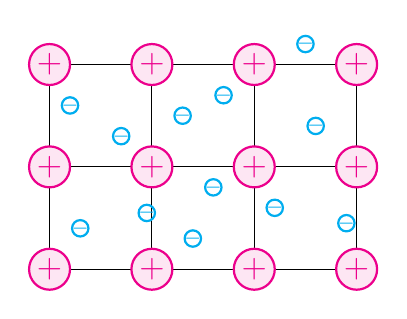
\begin{tikzpicture}[scale=1.3]
    \draw grid (3,2);
    \foreach \x in {0,...,3}{
      \foreach \y in {0,1,2}
      \draw[thick,magenta,fill=magenta!10] (\x,\y) circle (.2) node{\large$+$};
    }
    \begin{scope}[thick, cyan,fill=cyan!10]
      \draw (.2,1.6) circle (.08) node{\scriptsize$-$};
      \draw (.7,1.3) circle (.08) node{\scriptsize$-$};
      \draw (1.3,1.5) circle (.08) node{\scriptsize$-$};
      \draw (1.7,1.7) circle (.08) node{\scriptsize$-$};
      \draw (2.5,2.2) circle (.08) node{\scriptsize$-$};
      \draw (2.6,1.4) circle (.08) node{\scriptsize$-$};
      \draw (.3,.4) circle (.08) node{\scriptsize$-$};
      \draw (.95,.55) circle (.08) node{\scriptsize$-$};
      \draw (1.6,.8) circle (.08) node{\scriptsize$-$};
      \draw (1.4,.3) circle (.08) node{\scriptsize$-$};
      \draw (2.2,.6) circle (.08) node{\scriptsize$-$};
      \draw (2.9,.45) circle (.08) node{\scriptsize$-$};
    \end{scope}
  \end{tikzpicture}
  \caption{Atoms and electrons in metallic bonds}.
\end{figure}


\textbf{Conventional current} flows from the positive terminal (cathode) to the
negative terminal (anode). The flow  of current is assumed to be a continuous
function of time

We assume that positive charge carriers are all positively charged, and they
move with the same \textbf{drift velocity}. In most circuits, the drift
velocity is in the other of 0.1 to \SI1{\milli\metre\per\second}.

In reality, in a metal condcutor, electric current comes from motion of the
negatively-charged electrons moving in the \emph{opposite} direction of
convention current, called the \textbf{electron flow}, or
\textbf{electron current}, as shown in Fig.~\ref{fig:electron-flow}.
The electron's motion is chaotic, because as they move,
they collide with other electrons and with the atoms in the metal. The drift
velocity is the \emph{average} speed of the electrons. For circuit analysis,
we use the conventional current for simplicity.

\begin{figure}[ht]
  \centering
  \begin{subfigure}{.32\textwidth}
    \centering
    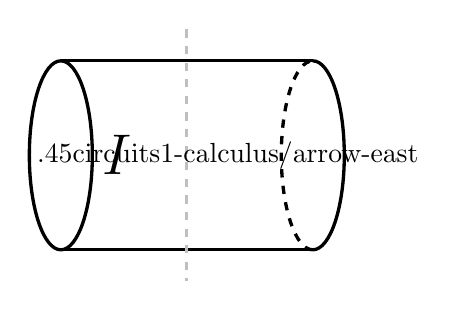
\begin{tikzpicture}[scale=.4]
      \draw[very thick] ellipse (1 and 3);
      \draw[very thick] (0,3)--+(8,0);
      \draw[very thick] (0,-3)--+(8,0);
      \draw[very thick] (8,-3) arc(-90:90:1 and 3);
      \draw[very thick,dashed] (8,-3) arc (270:90:1 and 3);
      \draw[very thick,dashed,lightgray] (4,4)--(4,-4);
      \node at (1.8,0){\huge$I$};
      \node at (5.3,0){\pic{.45}{circuits1-calculus/arrow-east}};
    \end{tikzpicture}
    \caption{Electric current modelled as continuously flow of charges}    
  \end{subfigure}
  \begin{subfigure}{.32\textwidth}
    \centering
    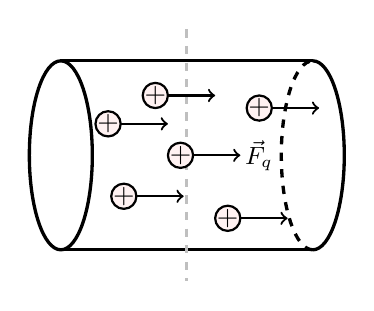
\begin{tikzpicture}[scale=.4]
      \draw[very thick] ellipse (1 and 3);
      \draw[very thick] (0,3)--+(8,0);
      \draw[very thick] (0,-3)--+(8,0);
      \draw[very thick] (8,-3) arc(-90:90:1 and 3);
      \draw[very thick,dashed] (8,-3) arc (270:90:1 and 3);
      \draw[very thick,dashed,lightgray] (4,4)--(4,-4);
        
      \draw[thick,fill=pink!20] (1.5,1) circle (.4) node{$+$};
      \draw[thick,->] (1.9,1)--+(1.5,0);

      \draw[thick,fill=pink!20] (2,-1.3) circle (.4) node{$+$};
      \draw[thick,->] (2.4,-1.3)--+(1.5,0);

      \draw[thick,fill=pink!20] (3,1.9) circle (.4) node{$+$};
      \draw[thick,->] (3.4,1.9)--+(1.5,0);

      \draw[thick,fill=pink!20] (3.8,0) circle (.4) node{$+$};
      \draw[thick,->] (4.2,0)--+(1.5,0) node[right=-2]{\small$\vec F_q$};

      \draw[thick,fill=pink!20] (5.3,-2) circle (.4) node{$+$};
      \draw[thick,->] (5.7,-2)--+(1.5,0);

      \draw[thick,fill=pink!20] (6.3,1.5) circle (.4) node{$+$};
      \draw[thick,->] (6.7,1.5)--+(1.5,0);
    \end{tikzpicture}
    \caption{Electric current modelled as discrete motion of ($+$) charges}
  \end{subfigure}
  \begin{subfigure}{.32\textwidth}
    \centering
    \begin{tikzpicture}[scale=.4]
      \draw[very thick] ellipse (1 and 3);
      \draw[very thick] (0,3)--+(8,0);
      \draw[very thick] (0,-3)--+(8,0);
      \draw[very thick] (8,-3) arc(-90:90:1 and 3);
      \draw[very thick,dashed] (8,-3) arc (270:90:1 and 3);
      \draw[very thick,dashed,lightgray] (4,4)--(4,-4);

      \draw[axes] (5,1)--(4,0)--(2.5,.5)--(.5,.8)--(0,0);
      \draw[thick,fill=pink!20] (5,1) circle (.4) node{\tiny$e^-$};

      \draw[axes] (8,-1)--(5,0)--(4.5,-.5)--(0,-.8); %--(0,0);
      \draw[thick,fill=pink!20] (8,-1) circle (.4) node{\tiny$e^-$};

      \draw[axes] (6.5,-1.8)--(4.2,-2)--(4,-1)--(2.5,-1.8)--(1,-1.5);
      \draw[thick,fill=pink!20] (6.5,-1.8) circle (.4) node{\tiny$e^-$};

      \draw[axes] (2.5,1.8)--(0,1.8);
      \draw[thick,fill=pink!20] (2.5,1.8) circle (.4) node{\tiny$e^-$};
    \end{tikzpicture}
    \caption{Electric current is actually the discrete motion of electrons}
    \label{fig:electron-flow}
  \end{subfigure}
  \caption{Modelling of electrical current in a metal conductor}
\end{figure}



\subsection{Electric Current in Solutions}

Materials that are formed by ionic bonds (e.g.\ sodium chloride, or table salt)
do not conduct electricity, but they can be dissolved, for example, in water,
and the solution containing the ions is now conductive. Positive ions move
towards negative terminal; while negative ions move towards positive terminal,
as shown in Fig.~\ref{fig:current-in-solutions}.
\begin{figure}[ht]
  \centering
  \begin{tikzpicture}[scale=.9]
    \draw[fill=cyan!20] rectangle (6,2.5);
    \foreach \x in {.4,5.6} \draw[line width=3] (\x,.5)--(\x,2);
    \draw[thick] (.4,1.25)--+(-1.5,0) node[left]{\large$+$};
    \draw[thick] (5.6,1.25)--+(1.5,0) node[right]{\large$-$};

    \begin{scope}[thick,magenta,fill=magenta!10]
      \draw[vectors] (1.2,2)--+(.5,0); \draw (1,2) circle (.2) node{$+$};
      \draw[vectors] (2.2,1.3)--+(.5,0); \draw (2,1.3) circle (.2) node{$+$};
      \draw[vectors] (3,.4)--+(.5,0); \draw (2.8,.4) circle (.2) node{$+$};
      \draw[vectors] (4.2,1.7)--+(.5,0); \draw (4,1.7) circle (.2) node{$+$};
      \draw[vectors] (3.5,1)--+(.5,0); \draw (3.3,1) circle (.2) node{$+$};
      \draw[vectors] (5,1.3)--+(.5,0); \draw (4.8,1.3) circle (.2) node{$+$};
    \end{scope}
    \begin{scope}[thick,cyan,fill=cyan!10]
      \draw[vectors] (1,1.2)--+(-.5,0);
      \draw (1.2,1.2) circle (.18) node{$-$};
      
      \draw[vectors] (1.7,.7)--+(-.5,0);
      \draw (1.9,.7) circle (.18) node{$-$};

      \draw[vectors] (2.8,2)--+(-.5,0);
      \draw (3,2) circle (.18) node{$-$};
      
      \draw[vectors] (3.1,1.6)--+(-.5,0);
      \draw (3.3,1.6) circle (.18) node{$-$};
      
      \draw[vectors] (4.5,.5)--+(-.5,0);
      \draw (4.7,.5) circle (.18) node{$-$};
    \end{scope}
  \end{tikzpicture}
  \caption{Motion of charges in a solution}
  \label{fig:current-in-solutions}
\end{figure}



%\subsection{Electric Field}
%Charge carriers move inside the circuit because they are subjected
%
%\subsection{Electric Current: Conventional vs.\ Electron Flow}
%The flow of electric current assumes the flow of \emph{positive} charges. We
%call this the \textbf{conventional current}:
%\begin{center}
%  \begin{tikzpicture}[scale=.8]
%    \draw (0,0)--(10,0);
%    \draw (0,1)--(10,1) node[midway,above]{$I\longrightarrow$};
%    \foreach \x in {1,3,...,9}{
%      \draw[thick,fill=pink!40] (\x,.5) circle (.25) node{$+$};
%      \draw[vector] (\x+.25,.5)--(\x+.75,.5);
%    }
%  \end{tikzpicture}
%\end{center}
%In a conducting wire, however, negatively charged electrons flow in the
%opposite direction. We call this the \textbf{electron current}:
%\begin{center}
%  \begin{tikzpicture}[scale=.8]
%    \draw (0,0)--(10,0);
%    \draw (0,1)--(10,1) node[midway,above]{$I\longrightarrow$};
%    \foreach \x in {1,3,...,9}{
%      \draw[thick,fill=blue!40!gray!20] (\x,.5) circle (.25) node{$-$};
%      \draw[vector] (\x-.25,.5)--(\x-.75,.5);
%    }
%  \end{tikzpicture}
%\end{center}
%Even though it is actually electron that are moving, we will continue to
%treat electric current as the flow of positive charges in the direction of
%the conventional current.




\section{Ohm's Law}

Georg Ohm discovered that when a current is passed through a piece of metal
conductor, the voltage (electric potential difference) $V$ across the two ends
of the metal is proportional to the amount of current ($I$) through it
(Fig.~\ref{fig:ohm1}).
\begin{figure}[ht]
  \centering
  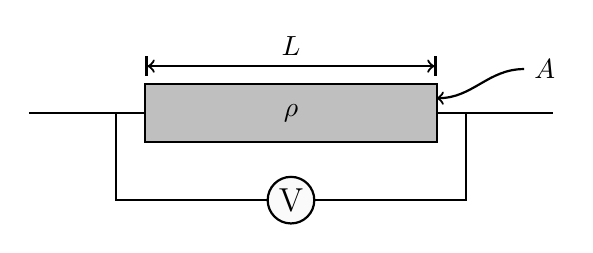
\begin{tikzpicture}[thick,scale=.37]
    \draw (-4,0)--(14,0);
    \draw (-1,0)--(-1,-3)--(11,-3)--(11,0);
    \draw[fill=lightgray] (0,-1) rectangle (10,1) node[midway]{$\rho$};
    \draw[fill=black!2] (5,-3) circle (.8) node{\large V};
    \draw[|<->|] (0,1.6)--(10,1.6) node[midway,above]{$L$};
    \draw[<-] (10,.5) to[out=0,in=180] (13,1.5) node[right]{$A$};
  \end{tikzpicture}
  \caption{Measuring voltage across a piece of meteal}
  \label{fig:ohm1}
\end{figure}


This is known as \textbf{Ohm's law}:
\begin{important-equation}
  V=IR
\end{important-equation}
The proportionality between voltage and current is called \textbf{resistance}.
We now know that electrical resistance is caused by the free electrons'
collisions with the atoms in the metal. The collisions transfer kinetic energy
from the electrons to the atoms. The atoms would then vibrate, and release
the additional energy in the form of electromagnetic radiation (as we have
learned, in Section~\ref{sec:heat-transfer}, is a form of heat transfer).
Note that Ohm's law is \emph{not} a fundamental law in physics; it only applies
to mostly metal conductors.



\subsection{Ohmic Devices}

Electrical devices where the relationship between voltage across the device and
the current through the device is linear are called \textbf{ohmic devices}.
Incandescent light bulbs and heating elements are examples of ohmic devices.
If we plot the current vs.\ voltage for the device, we would find a straight
line; the slope of the graph is the inverse of the resistance, as shown in
Fig.~\ref{fig:ohmic-relationship}.
\begin{figure}[ht]
  \centering
  \begin{subfigure}{.32\textwidth}
    \centering
    \begin{tikzpicture}
      \draw[function] (0,0)--(2.5,2.5)
      node[midway,right]{$\text{slope}=\dfrac1R$};
      \draw[axes] (0,0)--(3,0) node[right]{$V$};
      \draw[axes] (0,0)--(0,3) node[right]{$I$};
    \end{tikzpicture}
    \caption{Ohmic}
    \label{fig:ohmic-relationship}
  \end{subfigure}
  \begin{subfigure}{.32\textwidth}
    \centering
    \begin{tikzpicture}
      \draw[axes] (0,0)--(3,0) node[right]{$V$};
      \draw[axes] (0,0)--(0,3) node[right]{$I$};
      \draw[function,domain=0:2.45,smooth] plot(\x,.0008*\x^9);
    \end{tikzpicture}
    \caption{Non-ohmic}
    \label{fig:non-ohmic-relationship}
  \end{subfigure}
  \caption{Relationship between current and voltage for ohmic and non-ohmic
    devices.}
  \label{fig:i-vs-v-diagrams}
\end{figure}

\begin{remark}
  For clarification, the graphs in Fig.~\ref{fig:i-vs-v-diagrams} are plotted as
  $I$ vs.\ $V$. This is because we usually alter the voltage as an
  \emph{input}, and then measure the resulting current in the circuit as an
  \emph{output}. From this point of view, it makes sense that $V$ is the
  independent variable, and $I$ is the dependent variable. You can, of course,
  reverse the axes by plotting $V$ vs.\ $I$. In this case, across an ohmic
  device, the line would still be straight, but the slope would now be the
  resistance $R$.
\end{remark}



\subsection{Non-Ohmic Devices}

Loads that are \textbf{non-ohmic} do not obey Ohm's law; the relationship
between voltage and current is \emph{not} linear, as shown in
Fig.~\ref{fig:non-ohmic-relationship}. The majority of devices that we
encounter in circuits are non-ohmic. The include:
\begin{itemize}
\item Semi-conductor devices used for electronics
  \begin{itemize}
  \item Vacuum tubes
  \item Transistors
  \item Diodes (including light-emitting diodes, LEDs)
  \end{itemize}
\item Neon lights
\item DC motors
\end{itemize}
\begin{remark}
  A DC motor is ohmic if it is \emph{stalled}, i.e.\ current flows through it,
  but the motor shaft/axle does not turn. All of the energy is dissipated by
  the resistance in the wires inside the motor. A properly-operating DC motor
  is non-ohmic because as the armature turns, it generates a
  ``back \emph{emf}'' when the magnetic flux through the armature changes, as
  discussed in Faraday's law.
\end{remark}



\subsection{Resistance of a Conductor}
The resistance of a conductor is proportional to the resistivity $\rho$ and
its length $L$, and inversely proportional to the cross-sectional area $A$:
\begin{important-equation}
  R=\int\dl R=\rho\int_0^L\frac{\dl x}{A(x)}
\end{important-equation}


\begin{table}[ht]
  \centering
  \begin{tabular}{c|c|c}
    \rowcolor{cyan!30}
    Gauge & Diameter & $R/L$ \\
    \rowcolor{cyan!30}
    & (\si{\milli\metre}) & (\SI{e-3}{\ohm\per\metre})\\ \hline
    0  & \num{9.35} & \num{0.31} \\
    10 & \num{2.59} & \num{2.20} \\
    14 & \num{1.63} & \num{8.54} \\
    18 & \num{1.02} & \num{21.90} \\
    22 & \num{0.64} & \num{51.70}
  \end{tabular}
  \caption{Effects of cross sectional area on resistivity}
\end{table}

\begin{table}[ht]
  \centering
  \begin{tabular}{c|c}
    \rowcolor{cyan!30}
    Material & Resistivity $\rho$ (\si{\ohm.\metre}) \\ \hline
    silver    & \num{1.6e-8} \\
    copper    & \num{1.7e-8} \\
    aluminum  & \num{2.7e-8} \\
    tungsten  & \num{5.6e-8} \\
    Nichrome  & \num{100e-8} \\
    carbon    & \num{3500e-8}\\
    germanium & \num{.46} \\
    glass     & \num{e10} to \num{e14}
  \end{tabular}
  \caption{Resistivities of commany materials}
\end{table}

The resistivity of a material is proportional to the electric field $\bm E$
inside the wire and current density $\bm J$:
\begin{important-equation}
  \bm E=\rho\bm J
  \quad\text{or}\quad
  \rho=\left|\frac EJ\right|
\end{important-equation}
%\begin{center}
%  \begin{tabular}{l|c|c}
%    \rowcolor{pink}
%    \textbf{Quantity} & \textbf{Symbol} & \textbf{SI Unit} \\ \hline
%    Electric field & $\bm E$ & \si{\newton\per\coulomb} \\
%    Current density & $\bm J$ & \si{\ampere\per\metre\squared} \\
%    Resistivity & $\rho$ & \si{\ohm\metre}
%  \end{tabular}
%\end{center}
%\begin{itemize}
%\item In a conductor, the electrons are free to move, and the electric
%  field tend to be weak, and the resistivity is low.
%\item In an insulator, electrons cannot move easily, therefore the electric
%  field are generally strong, and the resistivity is high.
%\end{itemize}



\section{Power Dissipated by a Load}
Instantaneous power $P$ is the rate at which work $W$ is done, and from
electrostatics, the change in electric potential energy $\Delta E_q$ is
proportional to the amount of charge $q$ and the voltage $V$. This gives a very
simple expression for power through a resistor:  
\begin{equation}
  P=\diff Wt=\diff {E_q}t=\diff{(qV)}t=\left(\diff qt\right)V
  \;\rightarrow\;\boxed{P=IV}
\end{equation}
Combining Ohm's law with the above equation gives two additional expressions
for power through a resistor:
\begin{equation}
  \boxed{
    P=\frac{V^2}R
  }\quad\quad
  \boxed{
    P=I^2R
  }
\end{equation}



\section{Other Circuit Devices}

Aside from the necessary circuit devices,

For example, an energy sources may include:
\begin{figure}[ht]
  \centering
  \begin{subfigure}{.32\textwidth}
    \centering
    \begin{tikzpicture}[american voltages,thick]
      \draw (0,0) to[battery1,o-o] (2,0);
    \end{tikzpicture}
    \caption{Voltaic cell}
  \end{subfigure}
  \begin{subfigure}{.32\textwidth}
    \centering
    \begin{tikzpicture}[american voltages,thick]
      \draw (0,0) to[battery,o-o] (2,0);
    \end{tikzpicture}
    \caption{Voltaic pile (battery)}
  \end{subfigure}
  \begin{subfigure}{.32\textwidth}
    \centering
    \begin{tikzpicture}[american voltages,thick]
      \draw (0,0) to[pvsource,o-o] (2,0);
    \end{tikzpicture}
    \caption{Solar panel}
  \end{subfigure}

  \begin{subfigure}{.32\textwidth}
    \centering
    \begin{tikzpicture}[american voltages,thick]
      \draw (0,0) to[C,o-o] (2,0);
    \end{tikzpicture}
    \caption{Capacitor}
  \end{subfigure}
  \begin{subfigure}{.32\textwidth}
    \centering
    \begin{tikzpicture}[american voltages,thick]
      \draw (0,0) to[american voltage source,o-o] (2,0);
    \end{tikzpicture}
    \caption{DC voltage source}
  \end{subfigure}
  \begin{subfigure}{.32\textwidth}
    \centering
    \begin{tikzpicture}[american voltages,thick]
      \draw (9,0) to[sinusoidal voltage source,o-o] (11,0);
    \end{tikzpicture}
    \caption{AC voltage source}
  \end{subfigure}
  \caption{Examples of energy sources in an electric circuit}
\end{figure}

In voltaic cells and batteries, the \emph{emf} is controlled chemically; the
raw \emph{emf} output from each solar cell may vary, but the overall
\emph{emph} from a solar panel is generally controlled by a a device called a
\emph{maximum power-point tracker}; a generic DC voltage may not have a
constant \emph{emf}. A \textbf{capacitor} can also act as a energy source. When
a capacitor is charged---with charge $+Q$ on one plate, and $-Q$ on the other,
a voltage is generated, according to the equation $V=Q/C$ (studied in
Chapter~\ref{chapter:capacitors}).
%  \begin{center}
%    \begin{tikzpicture}[thick]
%      \draw (3,0) to[C,l=Capacitor,o-o] (5,0);
%    \end{tikzpicture}
%  \end{center}
%  Circuits with both resistors and capacitors will be studied next class.

Loads are devices that transforms the electrical energy in the circuit into
other forms of energy. Examples include those in
Fig.~\ref{fig:non-ohmic-loads}.
\begin{figure}[ht]
  \centering
  \begin{subfigure}{.24\textwidth}
    \centering
    \begin{circuitikz}[american voltages]
      \draw[thick] (0,0) to[R,o-o] (2,0);
    \end{circuitikz}
    \caption{Resistor}
  \end{subfigure}
  \begin{subfigure}{.24\textwidth}
    \centering
    \begin{circuitikz}[american voltages]
      \draw[thick] (3,0) to[bulb,o-o] (5,0);
    \end{circuitikz}
    \caption{Light bulb}
  \end{subfigure}
  \begin{subfigure}{.24\textwidth}
    \centering
    \begin{circuitikz}[american voltages]
      \draw[thick] (6,0) to[lamp,o-o] (8,0);
    \end{circuitikz}
    \caption{Lamp}
  \end{subfigure}
  \begin{subfigure}{.24\textwidth}
    \centering
    \begin{circuitikz}[american voltages]
      \draw[thick] (9,0) to[short,o-o] (11,0);
       \draw[very thick,fill=white] (9.35,-.2) rectangle (10.65,.2);
       \draw[very thick,fill=white] (10,0) circle (14pt) node{M};
    \end{circuitikz}
    \caption{DC motor}
  \end{subfigure}
  \caption{Non-ohmic loads}
  \label{fig:non-ohmic-loads}
\end{figure}
%  \begin{itemize}
%    \item Resistors, light bulbs and other lamps transform electrical energy
%      into heat, light and other forms of
%      \textbf{electromagnetic radiation}\footnote{Also known as
%      \textbf{electromagnetic waves}, or \textbf{EM waves}. They include radio
%      waves, microwaves, infrared radiation, visible light, ultraviolet (UV)
%      radiation, x-ray and gamma rays}
%    \item A motor converts electrical energy into kinetic energy of the motor
%      shaft and whatever objects are connected to it through an interaction
%      with a magnetic field inside the motor
%  \end{itemize}


There are also other circuit devices that are not strictly necessary, but are
very important/useful to ensure the reliable operation of an electrical
circuit. For example, a \textbf{fuse} will break (stopping current from
flowing) when the current through it exceeds its rating. A switch allows the
circuit to be manually turned on or off. (In the example, the switch is open
and no current flows through it.)
\begin{figure}[ht]
  \centering
  \begin{subfigure}{.35\textwidth}
    \centering
    \begin{tikzpicture}[thick,scale=1.2]
      \draw (0,0) to[fuse,o-o] (2,0);
    \end{tikzpicture}
    \caption{Fuse}
  \end{subfigure}
  \begin{subfigure}{.35\textwidth}
    \centering
    \begin{tikzpicture}[thick]
      \draw (0,0) to[short,o-] (.7,0) to[short,-*]
      +({.6*cos(40)},{.6*sin(40)});
      \draw (1.3,0) to[short,*-o] (2,0);
    \end{tikzpicture}
    \caption{Switch}
  \end{subfigure}
\end{figure}



%\section{Kirchhoff's Current Law}
%The electric current that flows into any junction in an electric circuit must
%be equal to the current which flows out.
%
%\begin{figure}[ht]
%  \centering
%  \begin{tikzpicture}[thick]
%%    \fill circle (.07);
%%    \draw (0,2)--(0,-1.5) to[R] (0,-3);
%%    \begin{scope}[rotate around={-60:(0,0)}]
%%      \draw (0,0)--(0,-1.5);
%%      \draw (0,-1.5) to[C,l=$C$,rotate around={-60:(0,-1.5)}] (0,-3);
%%    \end{scope}
%%    \draw[rotate=60] (0,0)--(0,-2);
%    \draw (.2,1) to[short,o-] (1.5,1)--(3.5,1)--(3.5,-.2);
%    \draw (1.5,1)--(1.5,-.2);
%    \draw (2.5,1)--(2.5,-.2);
%    \foreach \x in {1,...,3}
%    \draw[vector,red] (\x+.5,.9)--(\x+.5,.1) node[midway,left]{$I_{\x}$};
%    \draw[vector,red] (.4,1)--(1.3,1) node[midway,above]{$I$};
%  \end{tikzpicture}
%\end{figure}
%
%
%In the example on the left, with $I$ going into the junction, and $I_1$,
%$I_2$ and $I_4$ coming out, the current law says that
%\begin{equation}
%  I=I_1+I_2+I_3
%\end{equation}
%Basically, it means that there cannot be any accumulation of charges
%anywhere in the circuit. The law is a consequence of conservation of charge.
  


\section{Measuring Devices}

A \textbf{voltmeter} (Fig.~\ref{fig:voltmeter}) is used to measure the voltage
across two points in a circuit. To measure the voltage across a load, it is
placed in \emph{parallel} with a load. % to measure the voltage across it.
An ideal voltmeter has infinite resistance ($R=\infty$) and no current through
it ($I=0$).

An \textbf{ammeter} (Fig.~\ref{fig:ammeter}) is used to measure the current
across a point in the circuit. It is placed in \emph{series} with a load to
measure the current through it. An ideal ammeter has zero resistance ($R=0$),
thus it does not alter the flow of current in the circuit

An \textbf{ohmmeter} is used to measure the resistance of a particular load.
It is placed in \emph{parallel} with a load.
%to measure  the resistance across the load.
It can only be used when there is no active current in the circuit.
\begin{figure}[ht]
  \centering
  \begin{subfigure}{.32\textwidth}
    \centering
    \begin{tikzpicture}[scale=1.5]
      \draw[thick] (.2,0) to[R,l=$R$] (2.8,0);
      \draw[thick] (.7,0) to[short,*-](.7,-.8)--(2.3,-.8) to[short,-*] (2.3,0);
      \draw[very thick,fill=white] (1.5,-.8) circle (.3) node{V};
    \end{tikzpicture}
    \caption{Voltmeter}
    \label{fig:voltmeter}
  \end{subfigure}
  \begin{subfigure}{.32\textwidth}
    \centering
    \begin{tikzpicture}[scale=1.5]
      \draw[thick] (0,0) to[short] (1,0) to[R,l=$R$] (2.8,0);
      \draw[very thick,fill=white] (.7,0) circle (.3) node{A};
    \end{tikzpicture}
    \vspace{.47in}
    \caption{Ammeter}
    \label{fig:ammeter}
  \end{subfigure}
  \begin{subfigure}{.32\textwidth}
    \centering
    \begin{tikzpicture}[scale=1.5]
      \draw[thick] (0,0) to[R,l=$R$] (3,0);
      \draw[thick] (.7,0) to[short,*-] (.7,-.8)--(2.3,-.8) to[short,-*](2.3,0);
      \draw[very thick,fill=white] (1.5,-.8) circle (.3) node{$\Omega$};
    \end{tikzpicture}
    \caption{Ohmmeter}
  \end{subfigure}
  \caption{Circuit measuring devices}
\end{figure}

Voltmeters, ammeters and ohmmeters operate on the same principle using magnetic
effects inside the device, called a \textbf{galvanometer}. Modern voltmeters
are usually part of a \textbf{multi-meter} that also operates as an ammeter
and ohmmeter.
\begin{figure}[ht]
  \centering
  \pic{.4}{circuits1-calculus/voltmeter}
  \caption{A modern multimeter}
\end{figure}



\section{Kirchhoff's Laws}

\subsection{Kichhoff's Junction Law}
In the \textbf{junction law}, also known as the \textbf{current law}, the
electrical current that flows into any junction in a circuit must be equal to
the current which flows out.

\begin{figure}[ht]
  \centering
  \begin{tikzpicture}[scale=1.2]
    \draw[thick] (1,1) to[short,o-*] (1,0)--(0,0)--(0,-.7) to[R] (0,-2);
    \draw[thick] (1,-2) to[C] (1,-.7)--(1,0)--(2,0)--(2,-.7) to[L] (2,-2);
    \begin{scope}[ultra thick,red,->]
      \draw (1,.9)--(1,.1) node[midway,right]{$I$};
      \draw (.9,0)--(.1,0) node[midway,above]{$I_1$};
      \draw (1,-.1)--(1,-.9) node[midway,right]{$I_2$};
      \draw (1.1,0)--(1.9,0) node[midway,above]{$I_3$};
    \end{scope}
  \end{tikzpicture}
  \caption{An example of the junction law}
  \label{fig:junction-law}
\end{figure}
In the example in Fig.~\ref{fig:junction-law}, there are 4 paths to the
junction at the centre, with $I$ flowing into the junction, and $I_1$, $I_2$,
$I_3$ flowing out, then the junction law says that
\begin{equation*}
  I=I_1+I_2+I_3
\end{equation*}
regardless of what circuit devices those paths are connected to. In the
example, a resistor, a capacitor and an inductor\footnote{Inductor coils usee
magnetic field inside a solenoid to storage energy. It is \emph{not} part of
AP Physics 2} are joined at the junction. The junction law implies that there
must be no accumulation of charges anywhere in the circuit.



\subsection{Kichhoff's Voltage Law}

In the \textbf{voltage law}, the voltage changes around any closed loop in
the circuit must sum to zero, no matter what path you take through an
electrical circuit. In the example in Fig.~\ref{fig:voltage-law}, voltage gains
and losses from any of the loops always sum to zero:
\begin{align*}
  +\mathcal E-V_1-V_2 &= 0\quad\text{(ABCHA)}\\
  +\mathcal E-V_1-V_C &= 0\quad\text{(ABCDGHA)}\\
  +\mathcal E-V_1-V_L &=0\quad\text{(ABCDEFGHA)}
\end{align*}

\begin{figure}[ht]
  \centering
  \begin{tikzpicture}[scale=1.55,american voltages,thick]
    \draw (0,0) to[battery,l=$\mathcal E$] (0,1.5) to [R=$R_1$] (1.5,1.5)
    to[R=$R_2$] (1.5,0)--(0,0);
    \draw (1.5,1.5)--(2.5,1.5) to[C=$C$] (2.5,0)--(1.5,0);
    \draw (2.5,1.5)--(3.5,1.5) to[L=$L$] (3.5,0)--(2.5,0);
    \fill circle (.04) node[below left]{$A$};
    \fill (0,1.5) circle (.04) node[above left]{$B$};
    \fill (1.5,1.5) circle (.04) node[above]{$C$};
    \fill (2.5,1.5) circle (.04) node[above]{$D$};
    \fill (3.5,1.5) circle (.04) node[above]{$E$};
    \fill (3.5,0) circle (.04) node[below]{$F$};
    \fill (2.5,0) circle (.04) node[below]{$G$};
    \fill (1.5,0) circle (.04) node[below]{$H$};
  \end{tikzpicture}
  \caption{An example circuit with many elements}
  \label{fig:voltage-law}
\end{figure}


\begin{figure}[ht]
  \centering
  \begin{tikzpicture}[scale=1.75,american voltages,thick]
    \draw (1,1.5) to[short,o-] (1.5,1.5) to[R=$R_2$] (1.5,0)
    to[short,-o] (1,0);
    \draw (1.5,1.5)--(2.5,1.5) to[C=$C$] (2.5,0)--(1.5,0);
    \draw (2.5,1.5)--(3.5,1.5) to[L=$L$] (3.5,0)--(2.5,0);
  \end{tikzpicture}
\end{figure}
The voltage law can also show that the voltage across any circuit devices
connected in parallel (side by side) must be the same:
\begin{equation*}
  V_2=V_C=V_L
\end{equation*}


%\section{Kirchhoff's Voltage Law}
%The voltage changes around any closed loop in the circuit must sum to zero,
%no matter what path you take through an electric circuit. This also applies
%regardless of what circuit devices are along the path. In the example shown
%in Fig.~\ref{fig:kvl1}, a resistor $R$, capacitor $C$ and an inductor $L$ are
%in parallel with a battery of emf $\mathcal E$.
%
%\begin{figure}[ht]
%  \centering
%  \begin{tikzpicture}[scale=1.5,american voltages,thick]
%    \draw (0,0) to[battery1,l=$\mathcal E$] (0,1.5)
%    --(1.5,1.5) to[R=$R$] (1.5,0)--(0,0);
%    \draw (1.5,1.5)--(3,1.5) to[C,l=$C$] (3,0)--(1.5,0);
%    \draw (3,1.5)--(4.5,1.5) to[L,l=$L$] (4.5,0)--(3,0);
%    \node[below] at (0,0) {\small$A$};
%    \node[above] at (0,1.5) {\small$B$};
%    \node[above] at (1.5,1.5) {\small$C$};
%    \node[above] at (3,1.5) {\small$D$};
%    \node[above] at (4.5,1.5) {\small$E$};
%    \node[below] at (4.5,0) {\small$F$};
%    \node[below] at (3,0) {\small$G$};
%    \node[below] at (1.5,0) {\small$H$};
%  \end{tikzpicture}
%  \caption{A circuit with multiple circuit devices}
%  \label{fig:kvl1}
%\end{figure}
%
%Assume that the current flows clockwise and we draw a clockwise loop, we get
%\begin{equation}
%  \mathcal E-V_R=0\quad\rightarrow\quad\mathcal E-IR=0
%\end{equation}
  



\section{Resistors in Circuits}

\subsection{Resistors in Parallel}

\begin{figure}[ht]
  \centering
  \begin{tikzpicture}[thick]
    \draw (0,2) to[short,o-] (1,2) to[R=$R_1$] (1,0) to[short,-o] (0,0);
    \draw (1,2) to[short] (2.25,2) to[R=$R_2$] (2.25,0) to[short] (1,0);
    \draw (2.25,2) to[short] (3.5,2) to[R=$R_3\cdots$] (3.5,0)
    to[short] (2.25,0);
  \end{tikzpicture}
\end{figure}

The total current is the current through all the resistors, which can be
rewritten in terms of voltage and resistance using Ohm's law:
\begin{equation}
  I=I_1+I_2+I_3\cdots=\frac{V_1}{R_1}+\frac{V_2}{R_2}+\frac{V_3}{R_3}\cdots
\end{equation}    
Since $V_1=V_2=V_3=\cdots=V$ from the voltage law, we can re-write as
\begin{equation}
  I=\frac V{R_\text{parallel}}
  =V\left(\frac1{R_1}+\frac1{R_2}+\frac1{R_3}+\cdots\right)
\end{equation}
The inverse of the equivalent resistance for $N$ resistors connected in
parallel is the sum of the inverses of the individual resistances.
\begin{important-equation}
  \frac1{R_\text{parallel}}=\sum_i^N\frac1{R_i}
\end{important-equation}
As the number of resistors in parallel increase, the equivalent resistance
\emph{decreases} because this effectively increases the cross-sectional
area of the resistor.




\subsection{Resistors in Series}

\begin{figure}[ht]
  \centering
  \begin{tikzpicture}[thick]
    \draw (0,0) to[R=$R_1$,o-] (2,0) to[R=$R_2$] (4,0) to[R=$R_3$,-o] (6,0);
  \end{tikzpicture}
\end{figure}

The analysis for resistors in series is similar (but easier). From the current
law, the current through each resistor is the same:
\begin{equation}
  I_1=I_2=I_3=\cdots=I
\end{equation}
And the total voltage drop across all resistor is therefore:
\begin{equation}
  V=V_1+V_2+V_3+\cdots=I(R_1+R_2+R_3+\cdots)
\end{equation}
The equivalent resistance of loads is the sum of the resistances of the
individual loads.  
\begin{important-equation}
  R_\text{series}=\sum_{i=1}^NR_i
\end{important-equation}
Increasing the number of resistors in series \emph{increases} the equivalent
resistance because this effectively increases the length of the resistor.



%\section{Example Problem (Simple)}
%  A simple circuit analysis problem will involve one voltage source and
%  resistors connected, some in parallel, and some in series. Below is a typical
%  example:
%
%  \vspace{.2in}
%  
%    \begin{tikzpicture}[scale=.8,american voltages]
%      \draw(0,0) to[R=2<\ohm>](0,2) to[battery=100<\volt>] (0,4) to[short]
%      (1,4) to [R=10<\ohm>] (3,4)--(3,4.5) to[R=40<\ohm>] (5,4.5)
%      to[short] (5,4) to[short] (5.5,4)--(5.5,0)--(0,0);
%      \draw(3,4)--(3,3.5) to[R,l_=10<\ohm>] (5,3.5)--(5,4);
%      \draw[dashed] (-1.8,0.25) rectangle(0.6,3.75);
%    \end{tikzpicture}

%    Two \SI{10}{\ohm} resistors and a \SI{40}{\ohm} resistor are connected as
%    shown to a \SI{100}{\volt} emf source with internal resistance
%    \SI{2}{\ohm}. How much power is dissipated by the \SI{40}{\ohm} resistor?
%    \begin{enumerate}[(A)]
%    \item\SI{160}{\watt}
%    \item\SI{40}{\watt}
%    \item\SI{400}{\watt}
%    \item\SI{5}{\watt}
%    \item\SI{500}{\watt}
%    \end{enumerate}
%  
%



\section{Tips for Solving ``Simple'' Circuit Problems}
  \begin{enumerate}
  \item Identify groups of resistors that are in parallel or in series, and
    find their equivalent resistance.
  \item Gradually reduce the entire circuit to one voltage source and one
    resistor.
  \item Using Ohm's law, find the current out of the battery.
  \item Using Kirchhoff's laws, find the current through each of the resistors.
  \end{enumerate}





\section{Multi-loop Circuit}
Some of these problems require you to solve a system of linear equations.
The following is a simple example with two voltage sources:
\begin{center}
  \begin{tikzpicture}[american voltages,scale=1.3,thick]
    \draw (0,0) to[battery,l=$\mathcal E_1$] (0,2) to[R,l=$R_1$] (2,2)
    to[R,l=$R_3$] (2,0)--(0,0);
    \draw (2,0)--(4,0) to[battery,l_=$\mathcal E_2$] (4,2)
    to[R,l_=$R_2$] (2,2);

    \draw[vector,red] (2,.4)--(2,0) node[midway,right]{$I_1+I_2$};
    \draw[vector,red] (.6,.4) ..controls (0,2) and (2,2).. (1.6,.4)
    node[midway,below]{$I_1$};
    \draw[vector,red] (3.4,.4) ..controls (4,2) and (2,2).. (2.4,.4)
    node[midway,below]{$I_2$};
  \end{tikzpicture}
\end{center}
In this case, we have to draw two loops of current.




%\section{A More Difficult Example}
%\begin{center}
%  \begin{tikzpicture}[american voltages,thick]
%    \draw (0,0) to[battery, l=$\mathcal E_1$] (0,2) to[R=$R_1$] (2,2)
%    to[R=$R_3$] (2,0)--(0,0);
%    \draw (2,0)--(4,0) to[battery,l_=$\mathcal E_2$] (4,2) to[R,l_=$R_2$]
%    (2,2);
%    \begin{scope}[vector,red]
%      \draw (2,.4)--(2,0) node[midway,right]{$I_1+I_2$};
%      \draw (.6,.4) ..controls (0,2) and (2,2).. (1.6,.4)
%      node[midway,below]{$I_1$};
%      \draw (3.4,0.4) ..controls (4,2) and (2,2).. (2.4,.4)
%      node[midway,below]{$I_2$};
%    \end{scope}
%  \end{tikzpicture}
%\end{center}
  
We split the circuit into two loops, and apply Kirchkoff's voltage in both:
\begin{align*}
  \mathcal E_1-I_1R_1-(I_1+I_2)R_3&=0\\
  \mathcal E_2-I_2R_2-(I_1+I_2)R_3&=0
\end{align*}
There are two equations and two unknowns ($I_1$ and $I_2$) which we can either
solve algebraically or numerically. %We can subtract
%  (2) from (1), then solve for $I_1$ and $I_2$:
%
%  \begin{equation}
%    I_1=\frac{V_1-I_2R_3}{R_1+R_3}
%    \quad\quad
%    I_2=
%    \frac{\left[V_2-\frac{(V_1-V_2)R_3}{R_1}\right]}
%         {\left[R_2+\frac{(R_1+R_2)R_3}{R_1}\right]}
%  }
(Try this at home as an exercise.)



%\section{As Difficult As It Gets}
%  
%    \begin{tikzpicture}[american voltages,scale=1.2,thick]
%      \draw (0,0)--(0,2) to[R=3<\ohm>] (0,4)
%      to[battery1,l=42<\volt>] (2,4) to[R=3<\ohm>] (4,4)--(4,2)
%      to[R=4<\ohm>](4,0)--(2,0) to[battery1,l=6<\volt>] (2,2)
%      to[R,l_=4<\ohm>] (0,2);
%      \draw (0,0) to[R,l_=6<\ohm>](2,0);
%      \draw (2,2) to[R,l_=6<\ohm>](4,2);
%      \uncover<2->{
%        \begin{scope}[vector,red]
%          \draw (.5,3.5) ..controls(4.75,4) and (4.75,2).. (.5,2.5)
%          node[midway,left]{$I_1$};
%          \draw (.6,.4) ..controls (0,2) and (2,2).. (1.4,.4)
%          node[midway,below]{$I_3$};
%          \draw (2.6,.4) ..controls (2,2) and (4,2).. (3.4,.4)
%          node[midway,below]{$I_2$};
%        \end{scope}
%      }
%    \end{tikzpicture}

%    \begin{itemize}
%    \item To solve this problem, we define a few ``loops'' around the circuit:
%      one on top, one on bottom left, and one on bottom right.
%    \item<2-> Apply the voltage law in the loops. For example, in the
%      lower left:
%
%      \begin{equation}
%        4(I_1-I_3)-6-6I_3=0
%      }      
%    \item<2-> Solve the linear system to find the current. If the current that
%      you worked out is negative, it means that you have the direction wrong.
%    \end{itemize}

